
Za razmijevanje potreba penjača potrebno je analizirati alate koje penjači koriste. Ta rješenja mogu se podijeliti u dvije glavne kategorije: tradicionalne tiskane vodiče i moderne digitalne platforme koje su odgovorile na neka od ograničenja tiskanih vodiča.

\section{Tradicionalni tiskani penjački vodiči}

Desetljećima su tiskani vodiči bili jedini dostupni izvor informacija za snalaženje na stijenama. Njihova temeljna vrijednost leži u detaljnom i strukturiranom prikazu informacija koje kreiraju iskusni penjači. 

Vodiči su gotovo uvijek organizirani hijerarhijski kako bi korisniku olakšali navigaciju. Na najvišoj razini, vodič je podijeljen na penjališta, primjerice Kalnik, Kanjon Čikola, Golubinjak. Ta penjališta su često označena na velikoj karti koja se nalazi na početku vodiča. Unutar svakog područja sadržaj se dalje raščlanjuje na pojedinačne sektore, odnosno manje odvojene dijelove stijene. Za svaki sektor pružaju se ključne logističke informacije poput detaljni opis prilaza, informacije o parkiranju, vrijeme potrebno za pristup, GPS koordinate te opće napomene poput osunčanost ili preporučeno doba godine za posjet. 
Središnji element svakog vodiča je vizualni prikaz smjerova, odnosno \textit{topo}, koji može biti u formi detaljnog crteža ili fotografije preko koje su ucrtane linije smjerova. Uz svaki smjer navode se podaci o smjeru poput naziv, težina, dužina smjera te eventualno napomene poput upozorenje na nestabilno kamenje sklono kidanju. Osim informativnih \textit{topo} prikaza, vodiči su često obogaćeni fotografijama penjača te pejzažnim forografijama. 


U pravilu svaki vodič pokriva specifično geografsko područje, od pojedinačnih penjališta do cijele regije. U Hrvatskoj, najpoznatiji primjer vodiča za veću regiju je vodič "Croatia" autora Borisa Čujića. Uz njega postoje i specijalizirani vodiči za pojedina penjališta poput Nacionalnog parka Paklenica ili za regiju Istre. (slika~\ref{fig:vodic_paklenica})

\begin{figure}[H]
    \centering
    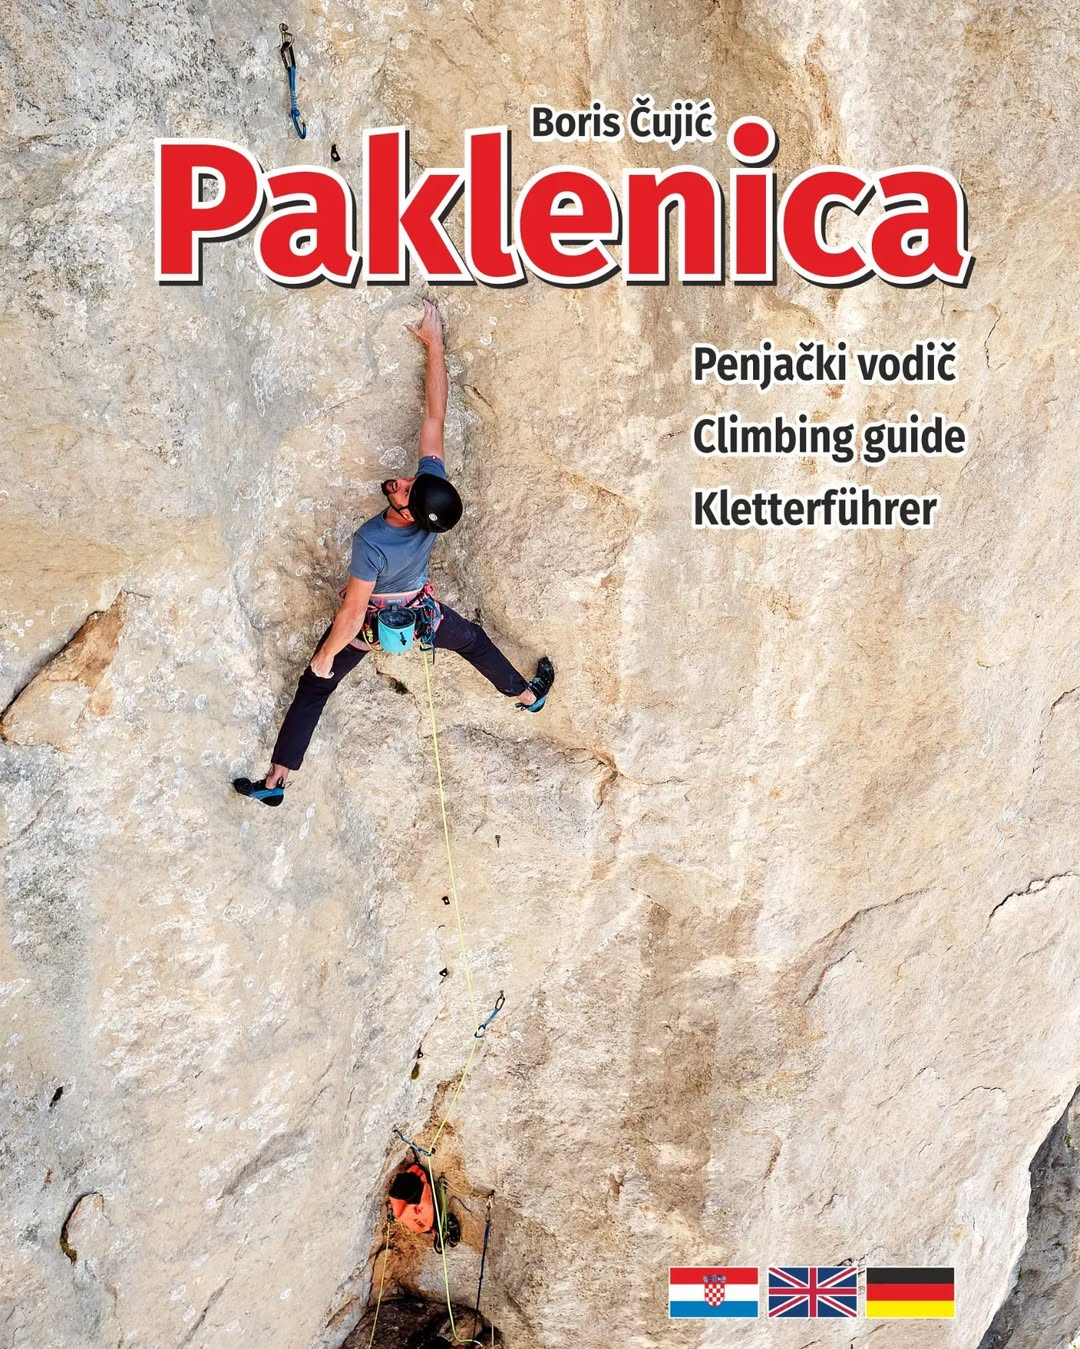
\includegraphics[width=0.6\textwidth]{images/analiza/vodic_paklenica.jpeg}
    \caption{Prikaz tiskanog penjačkog vodiča "Paklenica" autora Borisa Čujića}
    \label{fig:vodic_paklenica}
\end{figure}

Dodatnu složenost unose i izdanja stranih izdavača poput "Istra" autora Jurija Ravnika. Ova raznolikost izdavača dovodi do nedostatka konzistentnosti. Različiti vodiči koriste različite simbole, stilove i metodologije izrade \textit{topo} skica. Neki se oslanjaju na ručno crtane skice, a neki na fotografije. Bitno je spomenuti da se neujednačenost vidi i u težinama smjerova. Nije rijetko da isti smjer ima različite težine u različitim vodičima, što nije nužno posljedica promjene na stijeni ili novije izdanje, već subjektivna procjena autora. Ponekad se dogode i veće pogreške pri određivanju težine smjera što može dovesti do zabune. Sveukupno te nekonzistentnosti otežavaju snalaženje penjačima koji posjećuju različita područja i koriste vodiče različitih autora. 




\section{Digitalne platforme}

Ograničenja u tiskanim vodičima dovela su do pojave digitalnih platformi koje su omogućile veću dostupnost i ažurnost podataka. Dvije platforme, \textit{8a.nu} i \textit{27crags.com}, ističu se kao primjer rezličitih pristupa unutar digitalnog penjačkog svijeta. 

\subsection{8a.nu}

Platforma \textit{8a.nu} pokrenuta je 1999.\ godine i predstavlja jednu od najstarijih digitalnih platformi za penjanje. Njena glavna svrha nije funkcija terenskog vodiča, već uloga globalnog dnevnika uspona i sustava za rangiranje. 

\begin{figure}[H]
    \centering
    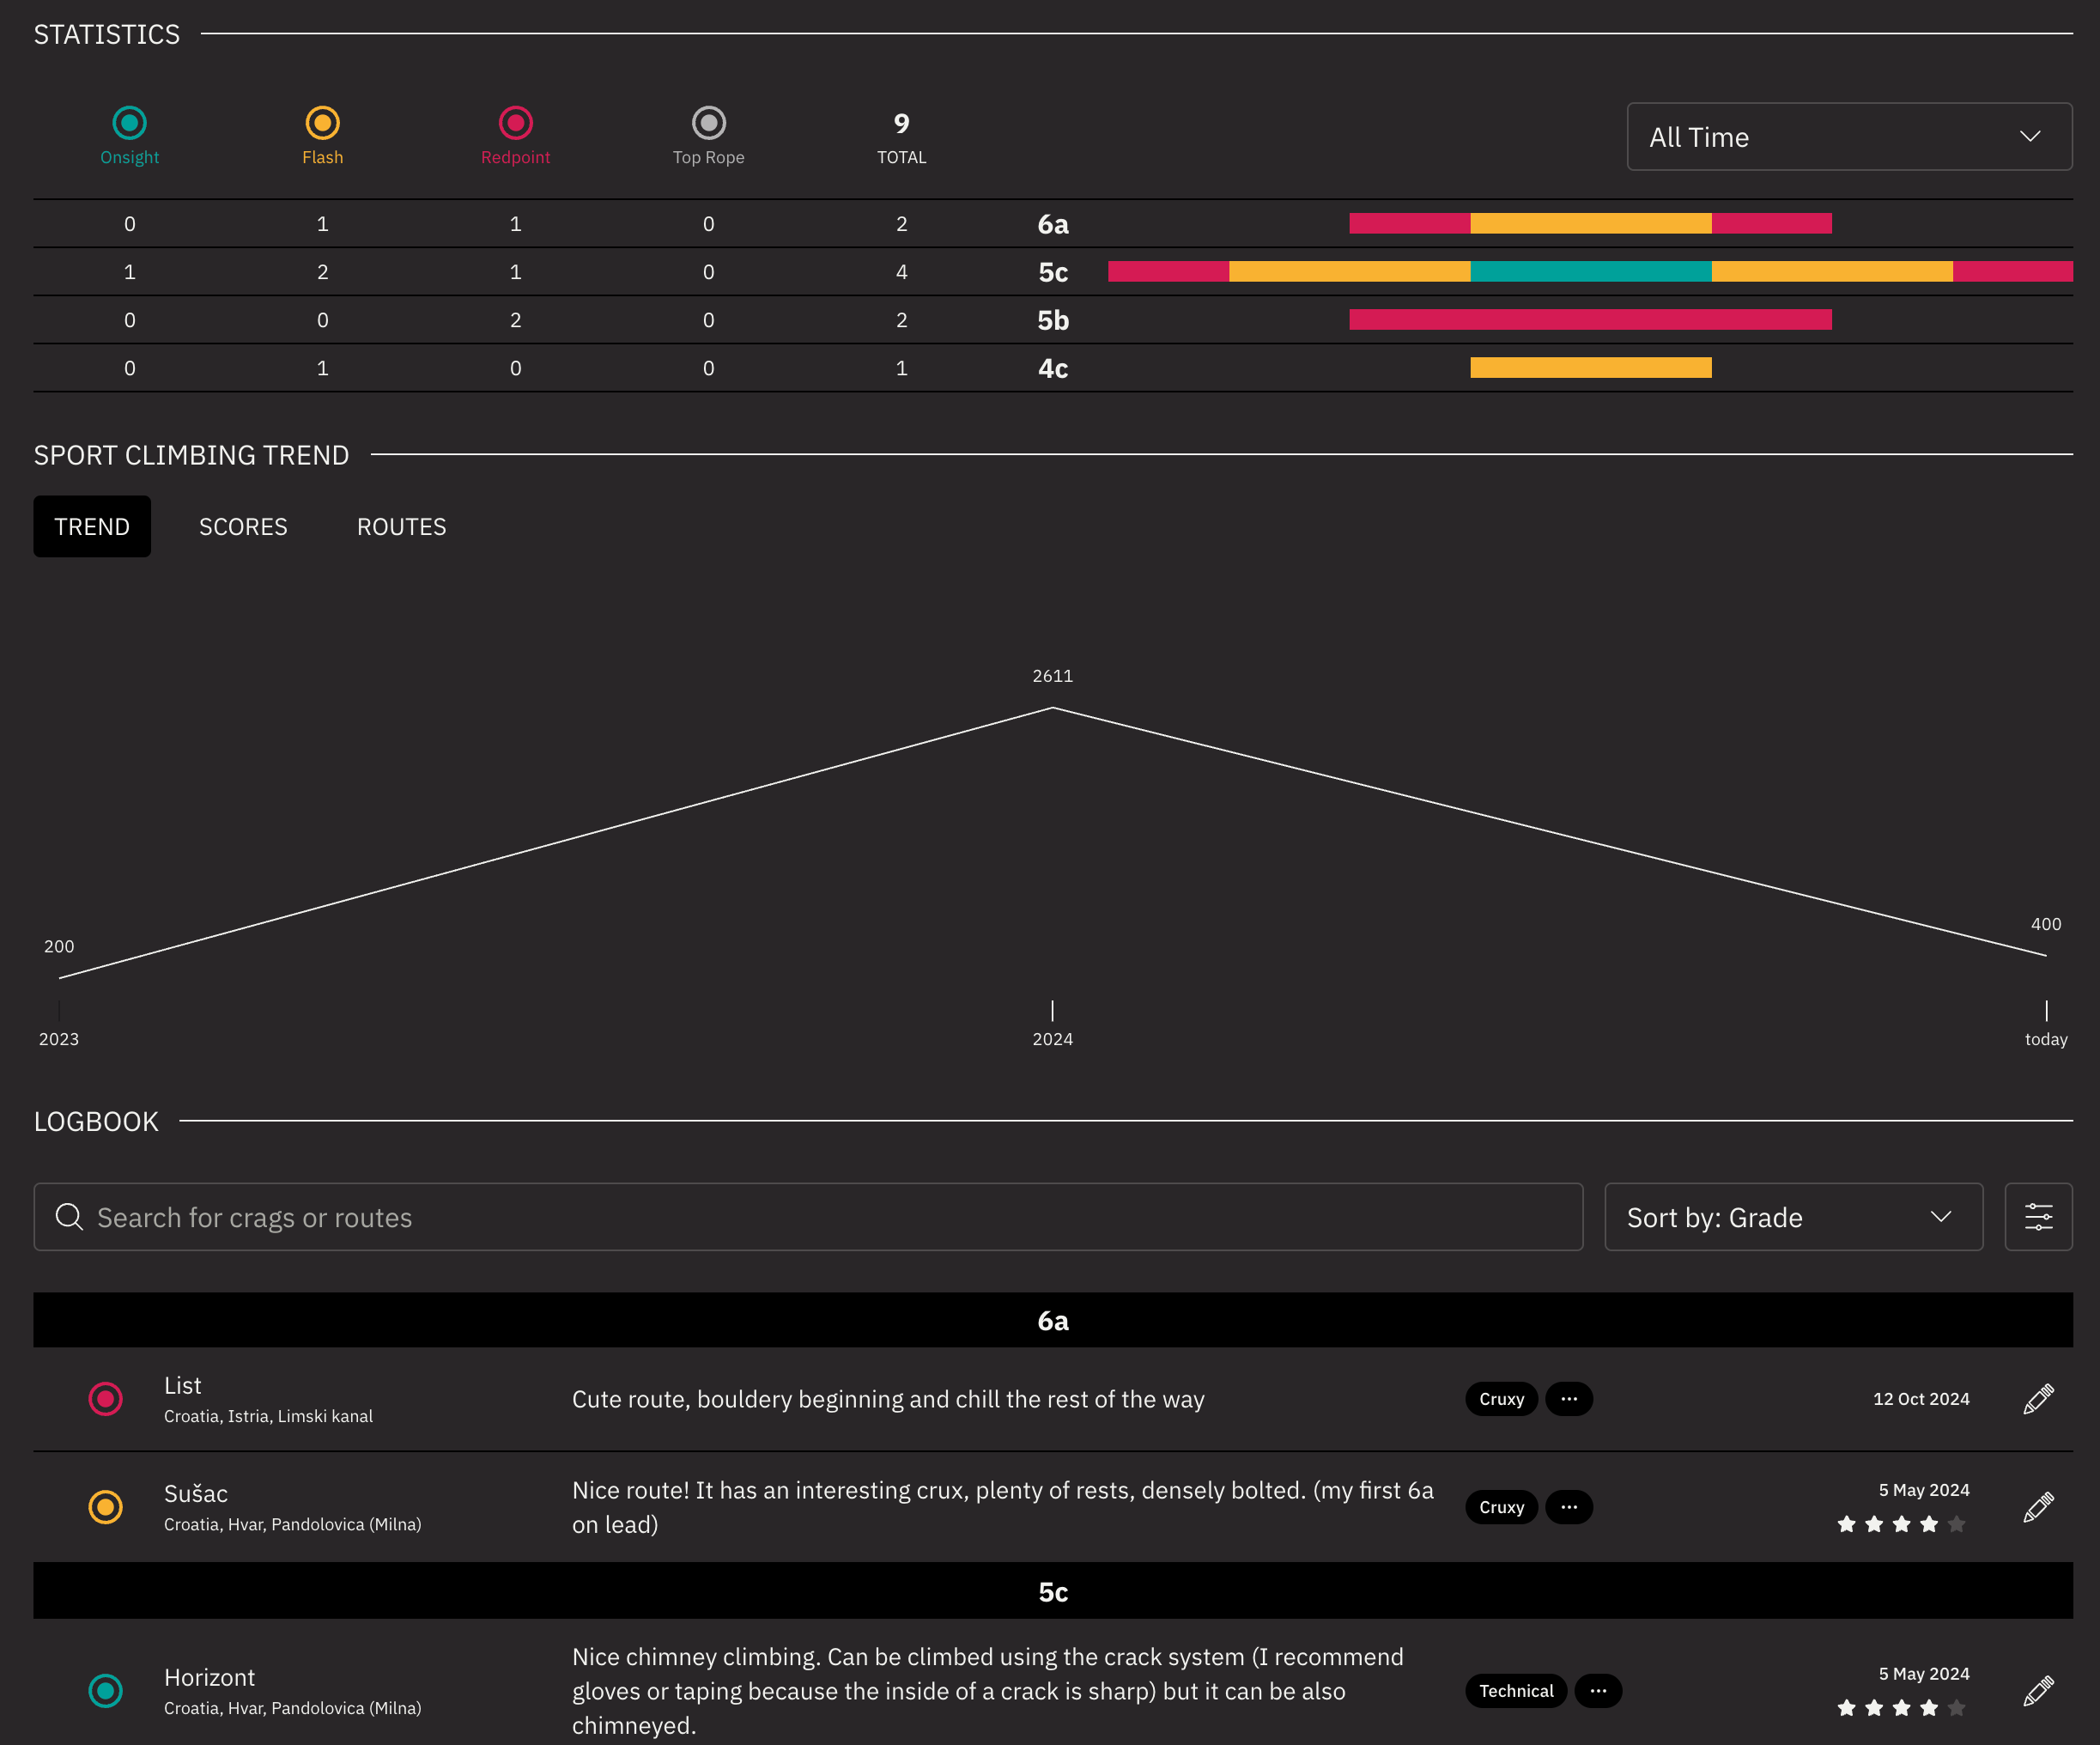
\includegraphics[width=0.8\textwidth]{images/analiza/8anu_logbook.png}
    \caption{Prikaz dnevnika uspona na platformi \textit{8a.nu}}
    \label{fig:8anu_logbook}
\end{figure}

Korisnici koriste platformu kako bi bilježili svoje ispenjane penjačke smjerove, navodeći stil uspona, predlagajući težine i komentare za smjerove (slika~\ref{fig:8anu_logbook}). Time se stvara velika, iako često nestrukturirana, baza podataka koja služi kao arhiv i statički resurs.



Ta društvena i natjecateljska komponenta je razlog njene dugovječnosti jer motivira penjače svih razina da upisuju svoje uspone. Platforma također nudi vjesti o značajnim usponima i forum za raspravu između penjača. Unatoč što aplikacija nudi \textit{topo} slike i hijerarhijski organizirana penjališta, njena primarna uloga je i dalje orijentirana prema društvenom aspektu. 
S nedavnim razvojem mobilne aplikacije, platforma je modernizirala korisničko sučelje i poboljšala dostupnost podataka na terenu nudeći opciju preuzimanja podataka na lokalni uređaj. Time je sustav upotrijebiv i u uvjetima bez signala.


\begin{figure}[H]
    \centering
    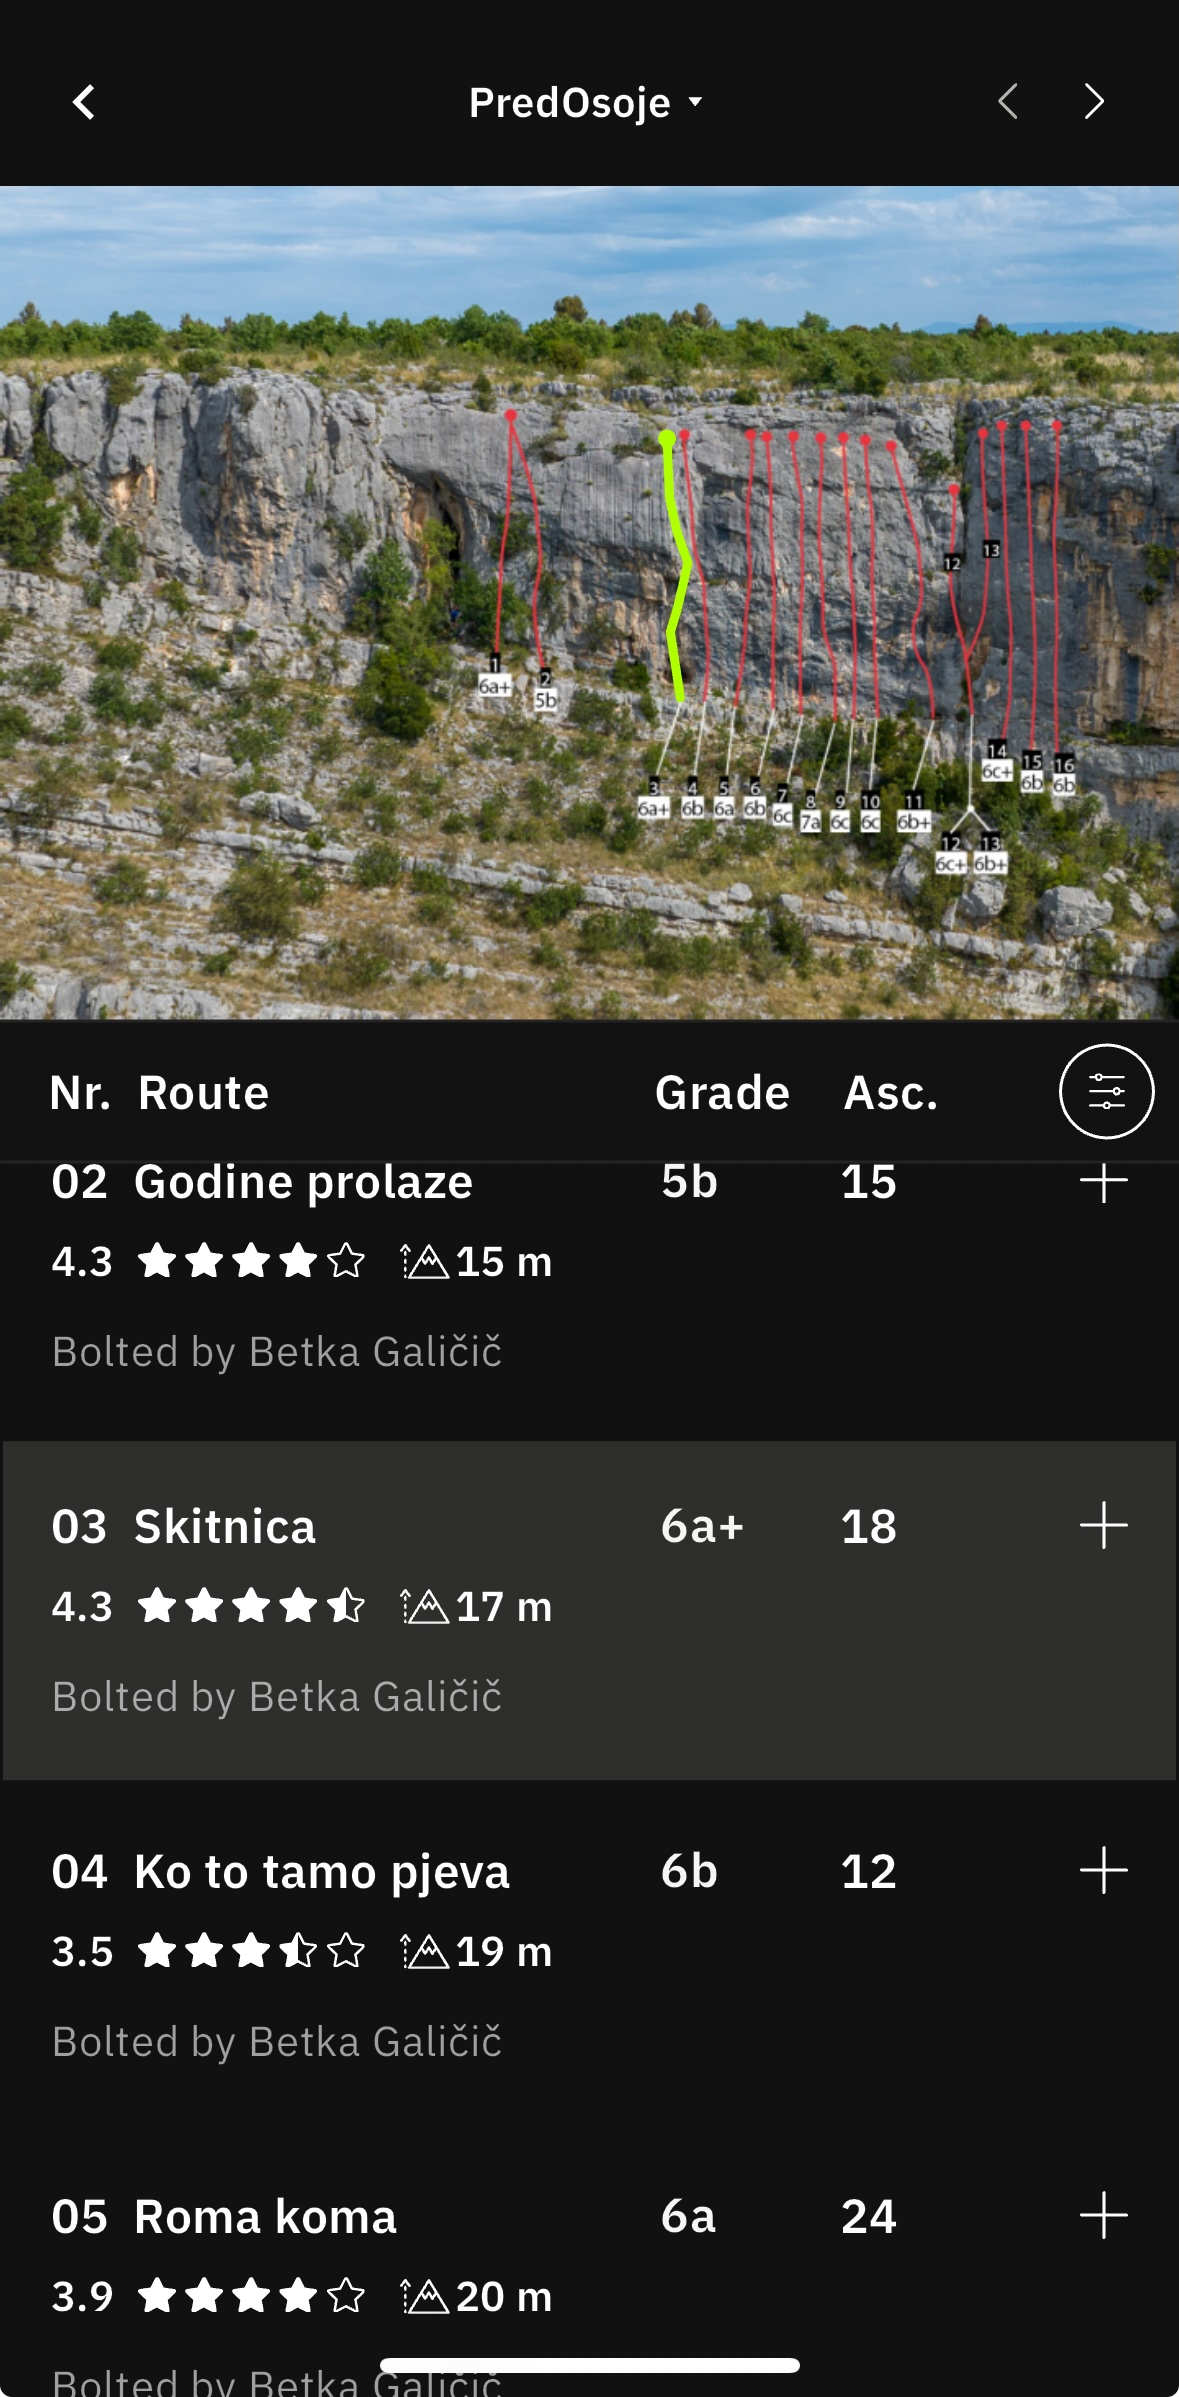
\includegraphics[width=0.4\textwidth]{images/analiza/8anu_mobile.jpg}
    \caption{Prikaz \textit{topo} skice na mobilnoj aplikaciji \textit{8a.nu}}
    \label{fig:8anu_mobile}
\end{figure}


Analizirajući \textit{8a.nu} aplikaciju kao alata za snalaženje na stijeni, njeni nedostaci u kontekstu vizalne navigacije su i dalje prisutni. Temeljni problem leži u samoj prirodi vizalnih prikaza. \textit{Topo} fotografije su često snimljene s velike udaljenosti kako bi obuhvatile cijeli sektor, zbog čega su ucrtane linije smjerova malene i nejasne. Ovaj problem postaje posebno izražen na sektorima s velikom gustoćom smjerova, kao što je prikazano na slici~\ref{fig:8anu_mobile}, gdje je teško precizno raspoznati pojedinačne linije i njihove početke. Dodatni problem predstavlja i neujednačena pokrivenost. Dok su međunarodno popularna penjališta dobro dokumentirane, manje ili lokalna penjališta, poput Kalnika u Hrvatskoj, nemaju dostupne \textit{topo} prikaze. Unatoč svojoj važnosti kao arhiva, platforma \textit{8a.nu} nije pouzdano rješenje za problem identifikacije smjerova na stijeni.

\subsection{27crags.com}

\textit{27crags.com} aplikacija predstavlja digitalnu platformu za penjače koje je izrađeno primarno s ciljem pružanja informacija o penjalištima i smjerovima. Ideja platforme \textit{27crags} je popisati što više penjališta i smjerova, a manji fokus je stavljen na društveni aspekt. \textit{Topo} skice su napravljene na sličan način kao i kod \textit{8a.nu} platforme, no društveni aspekt po pitanju uspona drugih penjača nije toliko u fokusu. Aplikacija nudi više informacija o penjalištima, poput parking lokacije sa detaljnim kartografskim prikazom.

Unatoč boljoj pokrivenosti penjališta, \textit{27crags} aplikacija također ima ograničenja po pitanju dvodimenzionalnog \textit{topo} prikaza (slika~\ref{fig:cikola_27crags_topo}) čime se ne riješava problem identifikacije penjačkih smjerova.

\begin{figure}[H]
    \centering
    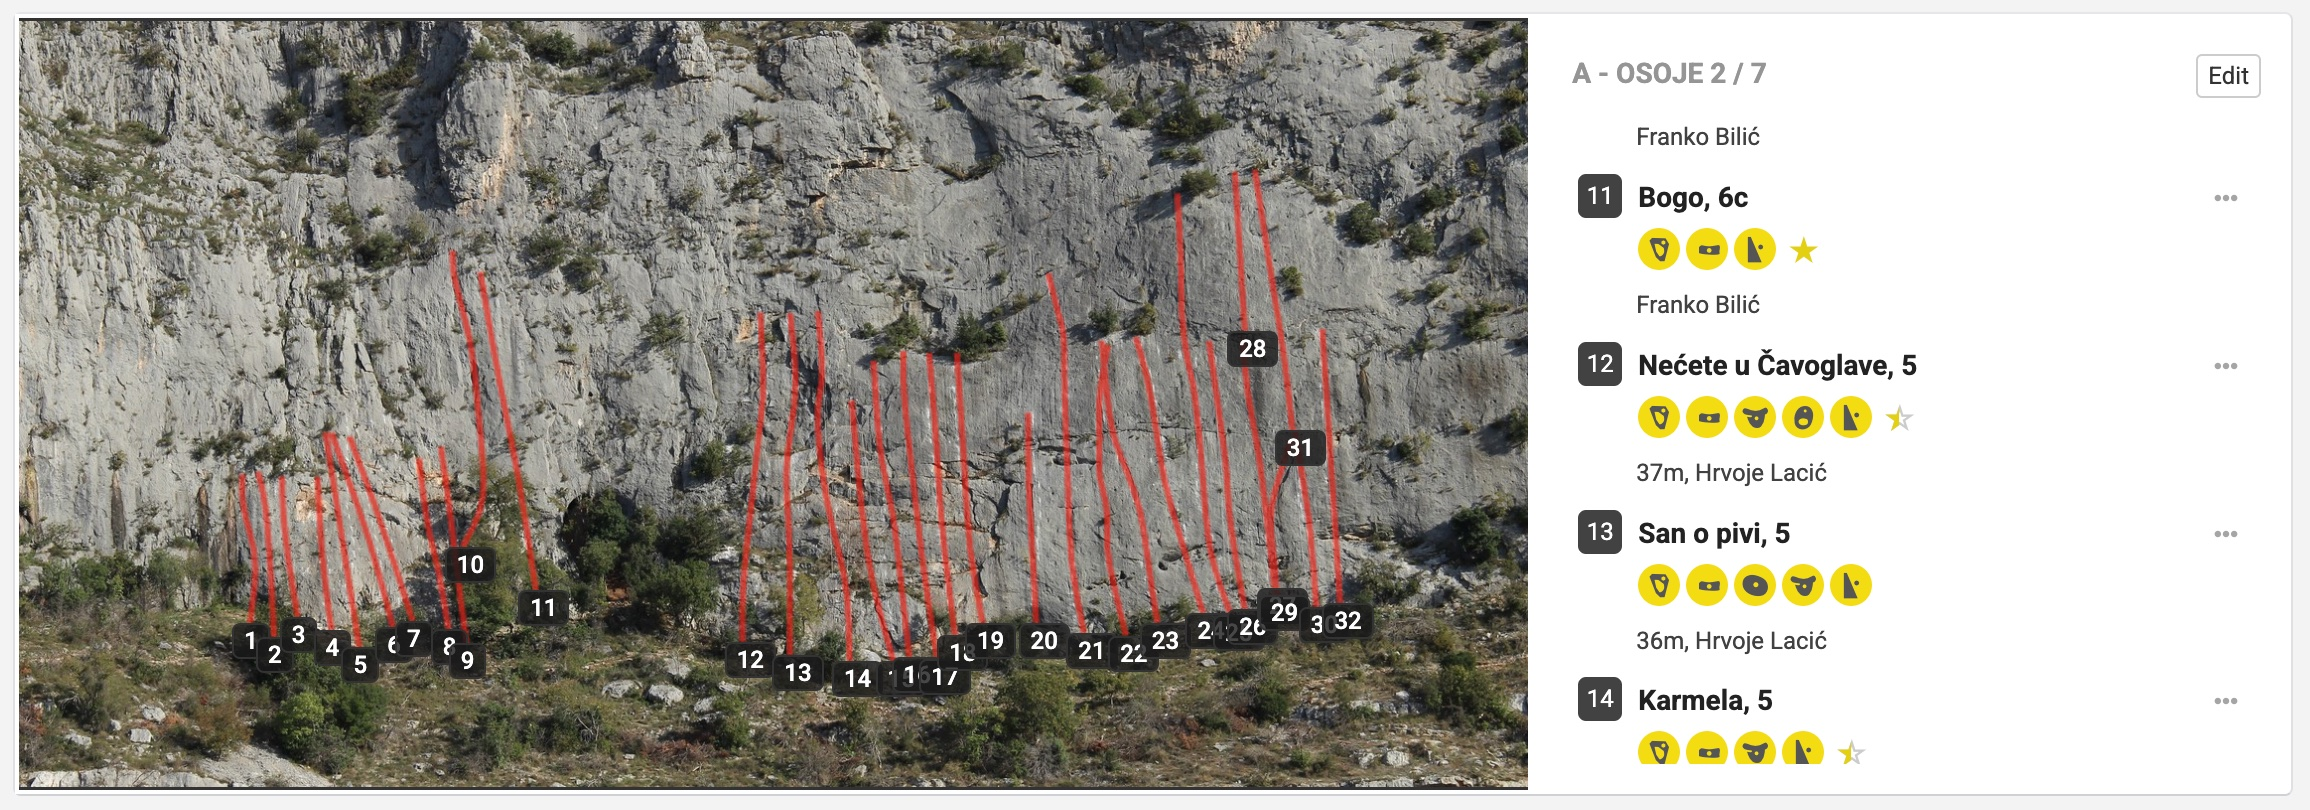
\includegraphics[width=1\textwidth]{images/analiza/cikola_27crags_topo.jpeg}
    \caption{Prikaz dvodimenzionalne \textit{topo} skice sa platforme \textit{27crags} za penjalište Čikola sektora Osoje}
    \label{fig:cikola_27crags_topo}
\end{figure}

\subsection{Ostale značajne digitalne platforme}

Uz navedene platforme, postoje i druge značajne digitalne platforme poput Mountain Project i KAYA. Mountain Project funkcionira kao sveobuhvatna, korisnički generirana baza podataka koja pokriva penjanje, planiniranje i druge aktivnost u prirodi. Razlika između Mountain Project i drugih aplikacija je što je izraziti fokus na rad bez internetske veze. Aplikacija zahtjeva od korisnika da unaprijed preuzme podatke za cijelu regiju kako bi mogao pristupiti sadržaju. Unatoč što to osigurava rad na lokacijama bez signala, platforma se i dalje oslanja na statične fotografije i korisničke opise.

KAYA je primjer novije platforme koja je popularna u svijetu \textit{bouldering} penjanja. Osim standardnih funkcionalnosti dnevnika uspona, KAYA omogućuje korisnicima objavu video sadržaja gdje pokazuju kako se penju određeni smjerovi, poznato pod nazivom \textit{beta} video.  Platforma je primarno usmjerena na američko tržište i dvoransko penjanje, zbog čega je njena pokrivenost manja od ostalih platformi, specifično za penjališta u Hrvatskoj. Unatoč inovativnom pristupu dijeljenja video sadržaja, KAYA ne nudi rješenje za identifikaciju penjačkog smjera na stijeni.


\section{Problem identifikacije penjačkog smjera: praktični izazovi}

Teorijska analiza nedostataka postojećih digitalnih aplikacija dobiva dodatno značenje kada se promotri stvarni proces identifikacije penjačkog smjera na terenu. Proces odabira penjačkog smjera može se podijeliti u dvije faze. Prva faza je identifikacija sektora u kojem se korisnik nalazi. Ova faza se generalno odvija prije nego što penjač dolazi ispred stijene. Penjač odabire sektor na temelju penjačkih smjerova koji se nalaze u sektoru, primjerice gleda težine smjerova, traži dulje penjačke smjerove ili traži sektor sa mnogo penjačkih smjerova.
\begin{figure}[H]
    \centering
    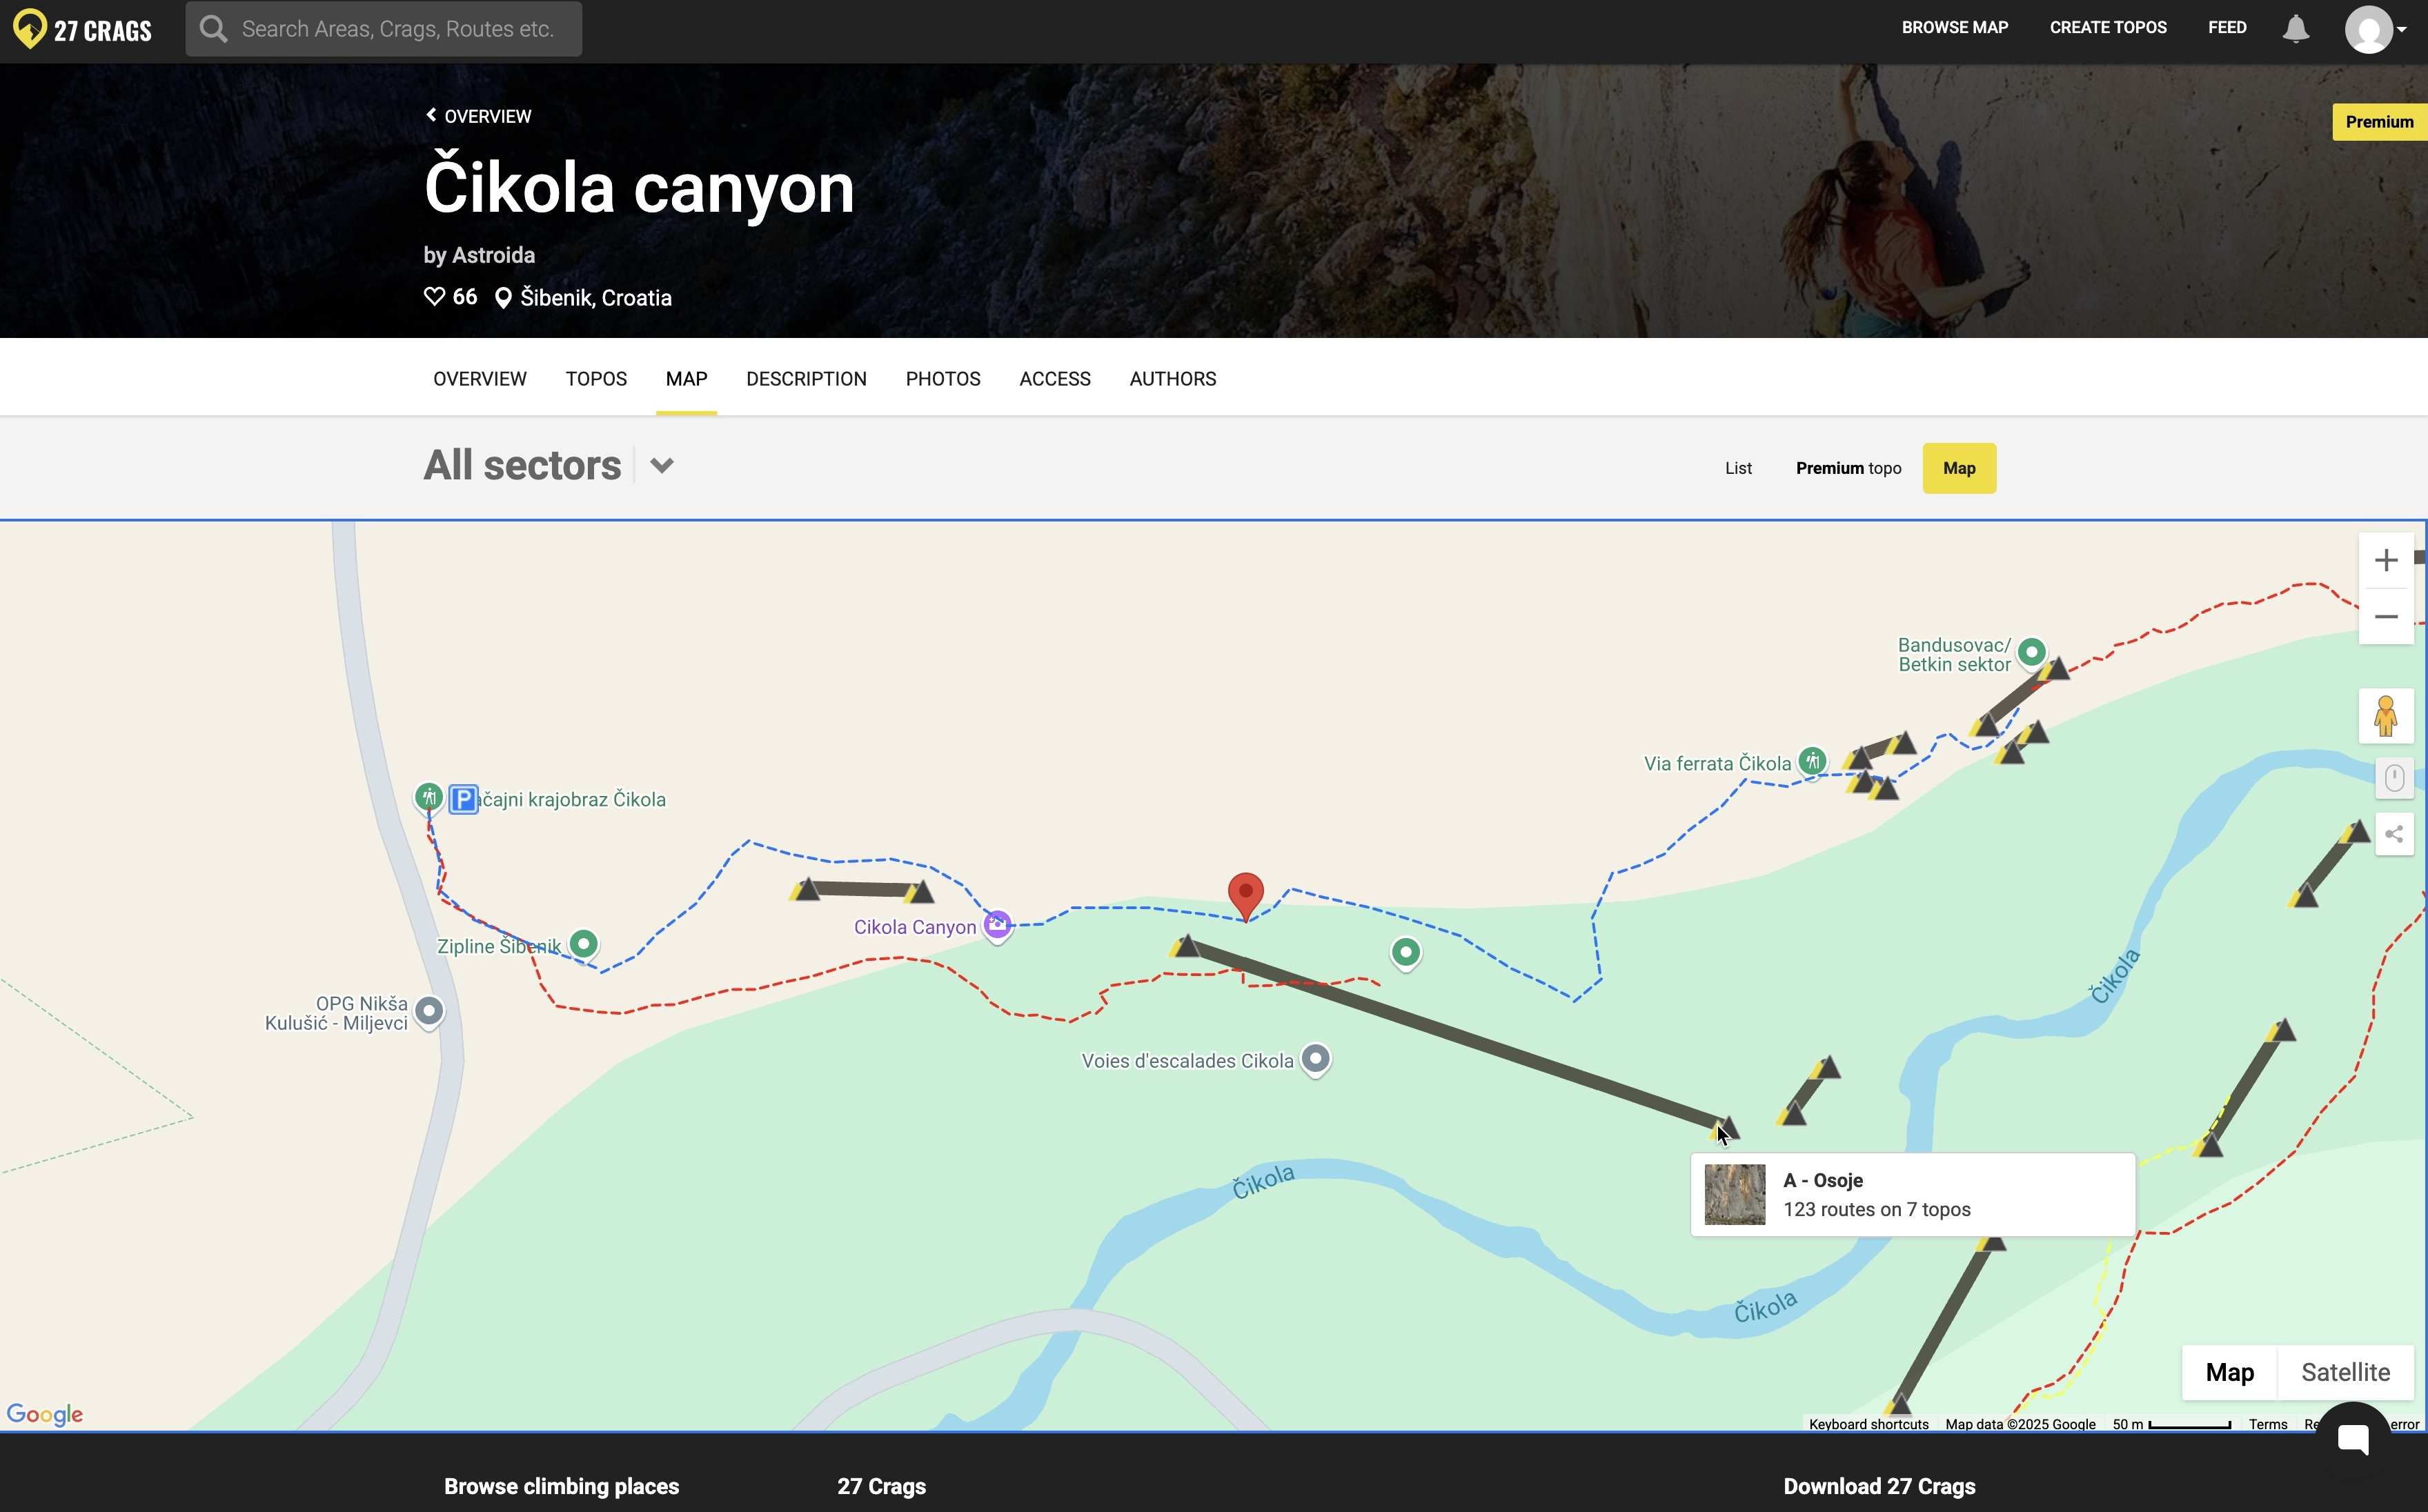
\includegraphics[width=0.9\textwidth]{images/analiza/cikola_27crags_map.jpeg}
    \caption{Prikaz geografske karte penjališta Čikola na platformi \textit{27crags}}
    \label{fig:cikola_27crags_map}
\end{figure} 
Problem odabira i pronalaženja sektora fizički i digitalni vodiči uspješno rješavaju. Svako penjalište sadrži geografsku kartu sa prikazom lokacija sektora. Slika~\ref{fig:cikola_27crags_map} prikazuje kako taj problem riješava platforma \textit{27crags}. Na karti su označeni sektori te prelaskom miša preko ikone pojavljuje se ime tog sektora. Fizički vodiči također sadrže kartu, no nije interaktivna kao što je na platformi \textit{27crags}. Svaki sektor sadrži listu penjačkih smjerova kojom penjač može odlučiti koji sektor želi posjetiti.

Dolaskom ispred stijene sektora kreće druga faza odabira penjačkog smjera i pojavljuje se problem identifikacije penjačkog smjera. Slika~\ref{fig:cikola_27crags_topo} predstavlja \textit{topo} sliku kojom se penjač koristi kako bi identificirao penjački smjer na stijeni.

\begin{figure}[H]
    \centering
    \includegraphics[width=0.8\textwidth]{images/analiza/cikola_fizicka_slika.jpg}
    \caption{Stvarna stijena na penjalištu Čikola sektora Osoje}
    \label{fig:cikola_fizicka_slika}
\end{figure} 

 Gledajući sliku~\ref{fig:cikola_fizicka_slika} teško je rasaznati gdje se penjač nalazi u odnosu na topo sliku i time je teško odrediti u koji penjački smjer penjač gleda. Često se traže distinktni elementi na stijeni poput velike rupe, nagle promjene u boji ili vegetacije, no ako je slika slikana iz velike udaljenost, to nije uvijek moguće. Cjelokupni proces je zahtjevan i podložan pogreškama te oduzima vrijeme koje bi se moglo iskoristiti za penjanje. Čak i uz pomoć fizičkih i digitalnih vodiča problem ostaje neriješen. Ta neefikasnost i nedostatak informacija predstavlja ključnu motivaciju za izradu sustava koji automatizira proces i pruža korisniku nedvosmislenu informaciju.